\chapter{SELFE Model}
\label{chap:selfe}
\section{Introduction}
\section{SELFE suite of tools}
The \acrfull{selfe} \citep{Zhang08} is a cross-scale 3D shallow water open source hydrodynamic model jointly 
developed by \acrfull{cmop} and \acrfull{vims}.

The main variables calculated by SELFE are the elevation of the free surface (stage), 
three-dimensional velocity and concentrations of salinity,
temperature and other scalar concentrations (only salinity is considered in this calibration), as well as turbulent quantities. Extensions in the SELFE suite use the flow field to calculate particle trajectories, sediment transport and nutrient availability. The input required by SELFE includes the initial state of the system and boundary time series
 representing fluxes and water surfaces at all the open boundaries. 

The underlying computational engine SELFE is a second-generation semi-implicit model sharing some of the 
algorithmic background of the \cite{Casulli99} family of models, which also includes UnTRIM and SUNTANS that have been
used before with some success on the Bay. SELFE's predecessor, ELCIRC \citep{Zhang04}, was perhaps the first open source model of this class to receive wide distribution. SELFE was devised to improve the depiction of 
bathymetry and salinity plume transport in realtime applications in the Columbia River region. 
SELFE shares some code with ELCIRC, but its discretization and solution scheme includes some 
innovations that make it more formally accurate. SELFE has also been parallelized and used by groups all over the world on a diverse
variety of high performance computers.

\begin{figure}
	\centering
		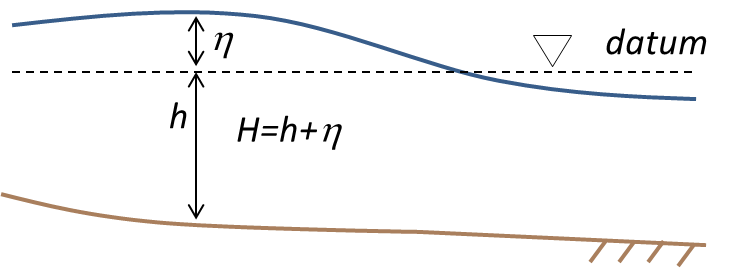
\includegraphics[scale=1.0]{image/depth_definition}
	\caption{Definition of bathymetric depth ($h$), elevation ($\eta$) and total depth ($H$) as used in SELFE.}
	\label{fig:depths}
\end{figure}

\section{Formulation}
\subsection{Equations of motion}\label{sec-1}
The formulation of SELFE is based on classic expressions of mass and momentum conservation within a shallow fluid,
as well as the transport equations for salt and heat. The three dimensional expressions of these laws of motion
involve much less reduction and averaging than one or two-dimensional models. However, 3D estuary-scale models
do invoke a standard set of assumptions that will be discussed in section \ref{sec-assump}.

The SELFE variant used in this equation is defined in a Cartesian (ie map projection) frame with
bathymetric depth $h$ and free surface $\eta$ defined relative to a fixed datum (NAVD 88 in our case) as shown 
in Figure \ref{fig:depths}. The total depth $H$ is the sum of bathymetric depth and free surface elevation.



The 3D continuity, depth-integrated mass conservation, and horizontal momentum conservation equations are given by:
\begin{align}
  %& \text{3D Continuity}& \nonumber \\
  \nabla \cdot \bs{u} &= 0 \label{3Dcon}&\\
  %& \text{Depth-integrated Continuity}& \nonumber \\
  \eta_t+\nabla \cdot \int_{-h}^\eta \bs{u} & = 0 \label{cont1} &\\
  %& \text{Momentum}& \nonumber \\
  \frac{D\bs{u}}{Dt} &= \explain{ -f\bs{k} \times \bs{u} }{\text{Coriolis}} 
	                      \; \explain{-\frac{1}{\rho_0} \nabla p_A}{\text{Atmos. pressure}}
												\; \explain{- \frac{g}{\rho_0} \int_z^\eta \nabla \rho d \xi}{\text{Baroclinic}}
	                      \; \; \; \explain{-g\nabla \eta}{\text{Gravity wave}} & \nonumber \\
	                      \; \; \; &\explain{+ \nabla \cdot (\mu \nabla \bs{u})}{\text{Horizontal diffusion}}
												\; \; \; \; \explain{+\frac{\pd}{\pd z}(\nu \frac{\pd \bs{u}}{\pd z})}{\text{Vertical diffusion}} \label{mom1}
	\end{align}
	with wind and bed stress boundary conditions at the surface and bottom of the water column:
	\begin{align}
	\nu \frac{\pd \bs{u}}{\pd z} &= \bs{\tau}_w \mbox{ at } z=\eta &\\
  \nu \frac{\pd \bs{u}}{\pd z} &= \chi \bs{u}_b \mbox{ at } z=-h &
\end{align}
where the variables and parameters are:
\begin{align*}
&\eta(x,y,t)  &\text{free surface elevation (m)} &\\
&\bs{u}(x,y,z,t)  &\text{horizontal velocity(m/s)}  &\\
&h(x,y)  &\text{bathymetric depth(m)} &\\
&w  & \text{vertical velocity (m/s)}  &\\
&f     & \text{Coriolis factor (s\textsuperscript{-1} )} & \\
&g     & \text{gravity (m/s\textsuperscript{2})} & \\
&\rho  & \text{water density (kg/m\textsuperscript{3})} & \\
&p_A(x,y, t) & \text{atmospheric pressure at the free surface (N m\textsuperscript{2})} & \\
&\nu    & \text{vertical eddy viscosity (m\textsuperscript{2}/s)} & \\
&\mu    & \text{horizontal eddy viscosity (m\textsuperscript{2}/s) }\\
&\kappa & \text{vertical eddy diffusivity, for salt and heat (m\textsuperscript{2}/s)} & \\
\end{align*}

and the labeled processes in the momentum equations include:
\begin{description}
    \item{Coriolis} an apparent force that results from writing equations on a rotating system (the earth) in a projected (x,y) coordinate system. The Coriolis force is most important in the ocean and near coast, less so in estuary or riverine systems. 
	  \item{Atmospheric pressure} This is the horizontal variation of pressure above the water.
		\item{Gravity wave} Pressure differences due to slope in the water surface are the main force that causes tide and flood propagation. 
	  \item{Baroclinic forcing} This is the driving mechanism for density-driven (exchange) flow, as
commonly found in estuaries, of which salinity intrusion is an example. Another example is gravity (dense) underflow. Due to this force, the horizontal gradient of the density field will initiate 3D flow that moves denser water under the lighter water and will lead to a two-layer flow structure commonly found in stratified estuaries. 
\end{description}

\subsubsection{Assumptions}\label{sec-assump}
The Reynolds averaged shallow water equations include some simplifications of the raw (Navier-Stokes) equations in order
to eliminate small scale terms and make the equations more tractable.
\begin{itemize}
\item {\em Free surface} The free surface is incorporated into the equations and results from the 
divergence of the horizontal flows. This simplification avoids a complex moving boundary problem at the water-atmosphere interface.
\item {\em Reynolds averaging} SELFE solves for velocity in a time-mean sense, averaged over small scale turbulence. Mixing induced by turbulent fluctuations 
is accounted for by relating the fluctuations to mean flow properties using a set of relations called the {\em turbulence closure}. 
\item {\em Boussinesq approximation} The Boussinesq approximation simplifies terms in the governing equations by considering the the effect of density differences due to soluble tracers (salt, temperature and sediment) only
in a single buoyancy term.
\item {\em Hydrostaticity} Most models in SELFE's class have both a hydrostatic and non-hydrostatic option. In hydrostatic mode, the model only considers pressure forces on a parcel of water arising only from the weight of the water and atmospheric pressure above, neglecting vertical momentum. 
The assumption can be relaxed by enabling non-hydrostatic pressure; however, due to the required resolution and computation time, 
this feature is not used at system scales in any model in the Bay-Delta.
\item In hydrostatic mode, volume conservation is first enforced over the water column using horizontal velocities into and out of the water column. Vertical velocity is implied in the equations and later inferred in a separate step that invokes the 3D continuity equation. 
\end{itemize}

\subsubsection{Roughness and friction}
In SELFE, resistance is introduced into the water column through the combination of the bottom stress (drag)
boundary condition and vertical turbulent momentum diffusion. The mechanism is less direct than the direct 
body force used in 1-D and 2-D models. [how does SELFE2D fit here?]

There are two options in the stipulation of the drag coefficient for each spatial location:
\begin{itemize}
	\item $C_d$ may be given directly
	\item $C_d$ may be inferred using an analytical description (logarithmic decay) of velocity in a viscous boundary layer. The parametrized form leads to a formula for $C_d$: 
	$C_d=[\frac{1}{\kappa_0}log(\frac{\delta}{z_0})]^{-2}$, where $\kappa_0$ is von Karman's constant, and $\delta$ is the thickness
of the bottom layer. In this case the calibration parameter is roughness ($z_0$) rather than drag.
\end{itemize}

Once drag is characterized at the bed, it is mixed vertically up the water column through a turbulent eddy diffusion, which is
labeled "vertical viscosity" in equation (\ref{mom1}) and shown visually in figure ****. The mixing of slower water into 
faster water has the effect of slowing the faster water down. Near the bed, this viscous process is the analog of
friction in a lower dimension model. Higher in the water column, the effect of eddy diffusion and location of the velocity
maximum are harder to predict.

In terms of calibration the above formulation leads to two sets of parameters that need to be estimated. The first is the
drag coefficient, which may take the form of $C_d$ or roughness $z_0$. In addition, an eddy diffusion coefficient 
has to be supplied -- this is not stipulated directly but rather emerges from the choice of turbulence closure, described in Section \ref{sec-tur}.

\subsection{Turbulence closure}\label{sec-tur}
The final component of vertical mixing is the turbulence closure, which is used to obtain an eddy viscosity coefficient
for the momentum equations and a vertical eddy diffusivity for the transport equations. 

We use the vertical component of Umlauf and Burchard's \cite{Umlauf2003}  generic length-scale model, a separate differential 
equation which is integrated "off-line" of the other equations based on values from the previous time step. 
The model is as follows:
\beqa
  \frac{D k}{D t}&=&\frac{\pd }{\pd z}\left( \nu_k^\Psi \frac{\pd k}{\pd z} \right)
  +\nu_t M^2+\nu_t^\theta N^2 -\epsilon \\
  \frac{D \Psi}{D t}&=& \frac{\pd }{\pd z}\left( \nu_\Psi \frac{\pd \Psi}{\pd z} \right)
    +\frac{\Psi}{k}(c_{\Psi 1}\nu_tM^2+c_{\Psi 3}\nu_t^\theta N^2-c_{\Psi 2}\epsilon F_{wall})
\eeqa
with natural b.c.:
\beq
   \left\{ \begin{array}{ll}
       \nu_k^\Psi \frac{\pd k}{\pd z} &=0, \mbox{ at } z=-h, \mbox{ or } \eta \\
       \nu_\Psi\frac{\pd \Psi}{\pd z} &= \kappa_0 n\nu_\Psi\frac{\Psi}{l} , \mbox{ at } z=-h \\
       \nu_\Psi\frac{\pd \Psi}{\pd z} &= -\kappa_0 n\nu_\Psi\frac{\Psi}{l} , \mbox{ at } z=\eta \\
           \end{array}
   \right.  \label{tur1}
\eeq
and essential b.c.:
\beq
   \left\{ \begin{array}{ll}
       k&=(c_\mu^0)^{-2} \nu|\frac{\pd \bs{u}}{\pd z}|, \mbox{ at } z=-h, \mbox{ or } \eta\\
       l&=\kappa_0 \D \\
       \Psi &= (c_\mu^0)^pk^m(\kappa_0 \D)^n
           \end{array}
   \right.  \label{tur2}
\eeq
where $k$ is the turbulent kinetic energy, $l$ is the mixing length, $c_{\Psi *}$ are some constants and $\Psi=(c_\mu^0)^pk^m l^n$ is a generic
length-scale variable, and $\D$ is the distance from 'walls' (i.e. surface and bottom). 

The turbulence production and dissipation terms are:
\beqa
  M^2&=&\left( \frac{\pd u}{\pd z}\right)^2+\left( \frac{\pd v}{\pd z}\right)^2 \\
  N^2 &=&-\frac{g}{\rho_0}\frac{\pd \rho}{\pd z} \\
  \epsilon &=& (c_\mu^0)^3k^{1.5} l^{-1}
\eeqa

In the code, the natural b.c. is applied first (see the FEM formulation below), and the essential b.c. is then used to overwrite the
boundary values of the unknown, as in the GOTM code. SELFE has been directly coupled to the GOTM model to take advantage of the latter.

Once the equations for turbulent kinetic energy mixing length have been updated, the 
values of eddy viscosity and eddy diffusivity used in the momentum and transport equations are obtained from the relations: 
\beqa
  \nu &=& \sqrt{2k}s_m l \\
  \kappa &=& \sqrt{2k}s_h l
\eeqa
where $s_m$ and $s_h$ are stability functions, such as those given by \citet{Kantha94}

With this step, the specification of turbulent mixing (and indirectly the mechanism of friction) is complete.




\subsection{Transport equation}
The advection-diffusion-reaction equation is the same in form for any tracer. 
SELFE uses it to track salt, temperature and sediment concentration and water quality constituents. 
The equation for a generic tracer $T$ is:
\beqa
  \frac{\pd T}{\pd t}+\nabla \cdot (\bs{u}T)
	&=& \frac{\pd }{\pd x} (\kappa_h \frac{\pd T}{\pd x}) + \frac{\pd }{\pd y} (\kappa_h \frac{\pd T}{\pd y})
	+\frac{\pd }{\pd z} (\kappa \frac{\pd T}{\pd z}) +\hat{Q},\label{tr1}\\
\eeqa
with vertical boundary conditions at the bed and free surface:
\beqa
  \kappa \frac{\pd T}{\pd z} &=& \hat{T}, \mbox{ at } z=\eta, \label{tr2} \\
  \kappa \frac{\pd T}{\pd z} &=& \hat{T_b}, \mbox{ at } z=-h, \label{tr3}
\eeqa
and concentration (Dirichlet, essential) boundary conditions at inflows and ocean boundaries.
where 
\begin{align*}
&T(x,y,z,t)  &\text{concentration of the tracer} &\\
&\bs{u}(x,y,z,t)  &\text{3D velocity (m/s)}  &\\
&\kappa_{h} &\text{horizontal diffusivity} (m^2s^{-1}) &\\
&\kappa   &\text{vertical diffusivity}(m^2s^{-1}) &\\
&\hat{Q}  & \text{mass source}  &\\
\end{align*}

and the 3D velocity $\bs{u}$ must be provided in a mass-conserving (divergence free) form:
\beq
  \nabla \cdot (\bs{u})=0 \label{tr5}
\eeq

Horizontal mixing of constituent concentration was ignored throughout our project, 
which is equivalent to $\kappa_h=0$. When shear in the main flow field is adequately
resolved, scaling arguments usually indicate that horizontal eddy diffusivity is very small
compared to the other terms and we assume that enough is introduced by the unavoidable horizontal
numerical diffusion introduced in solving the equations.




%
\subsection{Turbulence closure}\label{sec-tur}


We use the \citet{Umlauf2003} generic length-scale model:
\beqa
  \frac{\D k}{\D t}&=&\frac{\pd }{\pd z}\left( \nu_k^\Psi \frac{\pd k}{\pd z} \right)
  +\nu_t M^2+\nu_t^\theta N^2 -\epsilon \\
  \frac{\D \Psi}{\D t}&=& \frac{\pd }{\pd z}\left( \nu_\Psi \frac{\pd \Psi}{\pd z} \right)
    +\frac{\Psi}{k}(c_{\Psi 1}\nu_tM^2+c_{\Psi 3}\nu_t^\theta N^2-c_{\Psi 2}\epsilon F_{wall})
\eeqa
with natural b.c.:
\beq
   \left\{ \begin{array}{ll}
       \nu_k^\Psi \frac{\pd k}{\pd z} &=0, \mbox{ at } z=-h, \mbox{ or } \eta \\
       \nu_\Psi\frac{\pd \Psi}{\pd z} &= \kappa_0 n\nu_\Psi\frac{\Psi}{l} , \mbox{ at } z=-h \\
       \nu_\Psi\frac{\pd \Psi}{\pd z} &= -\kappa_0 n\nu_\Psi\frac{\Psi}{l} , \mbox{ at } z=\eta \\
           \end{array}
   \right.  \label{tur1}
\eeq
and essential b.c.:
\beq
   \left\{ \begin{array}{ll}
       k&=(c_\mu^0)^{-2} \nu|\frac{\pd \bs{u}}{\pd z}|, \mbox{ at } z=-h, \mbox{ or } \eta\\
       l&=\kappa_0 \D \\
       \Psi &= (c_\mu^0)^pk^m(\kappa_0 \D)^n
           \end{array}
   \right.  \label{tur2}
\eeq
where $k$ is the TKE, $l$ is the mixing length, $c_{\Psi *}$ are some constants and $\Psi=(c_\mu^0)^pk^m l^n$ is a generic length-scale variable.
The turbulence production and dissipation terms are:
\beqa
  M^2&=&\left( \frac{\pd u}{\pd z}\right)^2+\left( \frac{\pd v}{\pd z}\right)^2 \\
  N^2 &=&\frac{g}{\rho_0}\frac{\pd \rho}{\pd z} \\
  \epsilon &=& (c_\mu^0)^3k^{1.5} l^{-1}
\eeqa
In the code, the natural b.c. is applied first (see the FEM formulation below), and the essential b.c. 
 is then used to overwrite the boundary values of the unknown, as suggested by the \gls{gotm} implementation.

GOTM has also been coupled to SELFE, but the native (finite element) implementation is the one used for the Bay-Delta project.

\subsection{Vertical velocity closure}
The hydrostatic momentum equations are written in terms of horizontal velocities, combined with mass conservation over the water column. Often it is necessary to recover the compatible conservative 3D velocity field, either for diagnostic purposes or to feed into the transport equations. 

SELFE infers vertical velocities by integrating the 3D mass conservation equation (\ref{3Dcon})
from the bed to the free surface. The process is illustrated in Figure \ref{fig:vel_close}. Starting at the bed, a suitable boundary condition (e.g. zero flow) is assumed. This is combined with horizontal flows across the three vertical faces of the prism as well as the component of flow flows directed across the (very slightly tilted) top face of the
prism. Given that water is incompressible, what comes out must be the vertical component of flow up out of the top face. The
calculation then proceeds to the prism above.

\begin{figure}
	\centering
		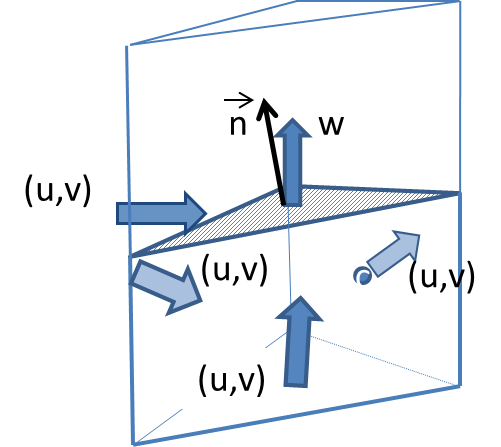
\includegraphics[scale=1.0]{image/vel_closure}
	\caption{First closure calculation on bottom prism. The horizontal velocities at the three vertical faces and the horzizontal component of velocity normal to the top face are shown and designated $(u,v)$. The vertical velocity $w$ is obtained from the 
	net flux. Movement of the S grid (typically a small fraction of a millimeter per time step) is not considered.}
	\label{fig:vel_close}
\end{figure}


\section{Discretization and data centering}
SELFE uses a triangular unstructured mesh in the horizontal direction and a bathymetry-conforming 
hybrid Z-S coordinate mesh \citep{Zhang08} in the vertical.

\subsection{Horizontal mesh}
The horizontal mesh is referred to as {\em unstructured} because the connectivity of the triangles 
is general and unconstrained. 
Unstructured grids incur some computational overhead because lists of neighbors must be tabulated as input and neighbors 
are not adjacent to one another in memory on the computer. The benefit, though, is that it is 
easy to represent complex shorelines with a fair amount of accuracy (see, for instance, Figure \ref{fig:hgrid}.

\begin{figure}
	\centering
		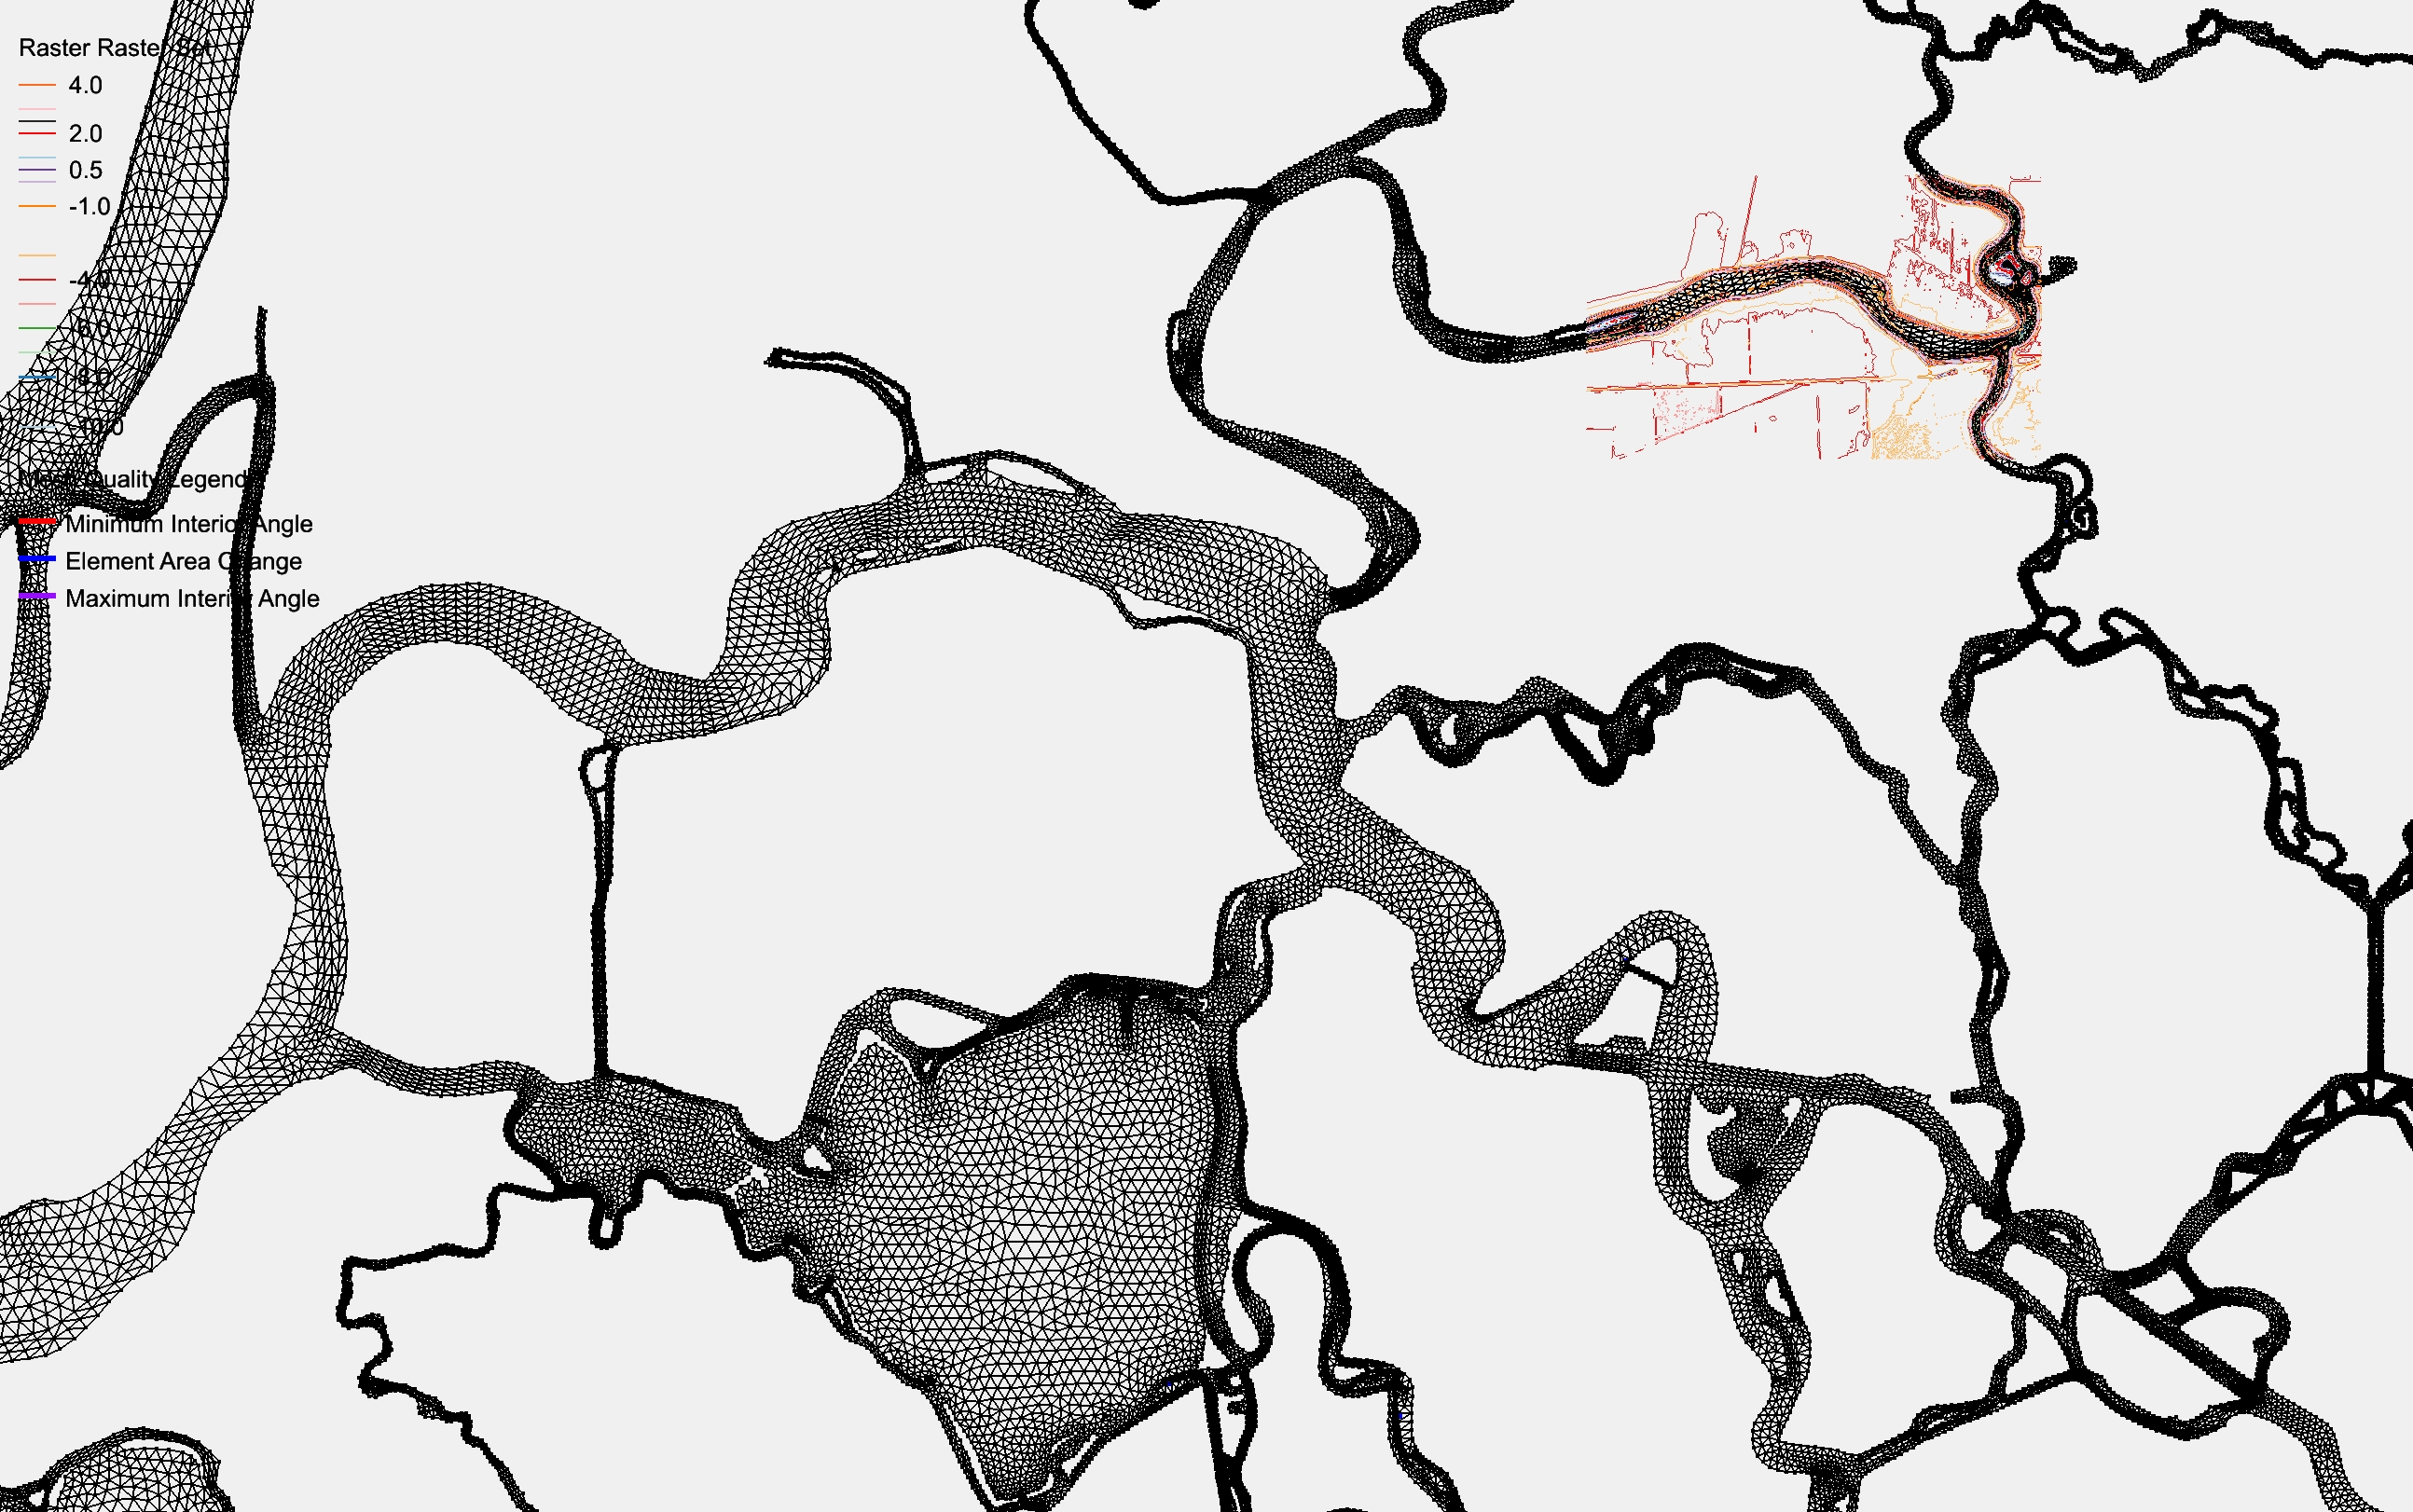
\includegraphics[width=\textwidth,clip,trim=3in 0in 2.5in 4.25in]{image/hgrid}
	\caption{Horizontal mesh near Franks Tract.}
	\label{fig:hgrid}
\end{figure}

\begin{figure}
	\centering
		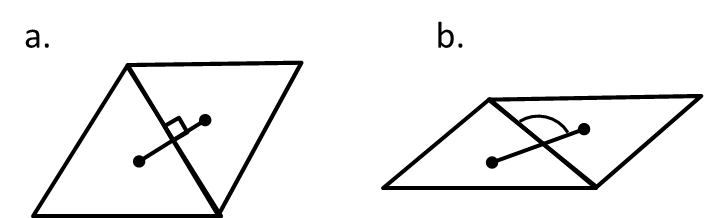
\includegraphics[scale=1.0]{image/ortho}
	\caption{a. Orothogonal triangular mesh. b. Non-orthogonal mesh with some skew.}
	\label{fig:ortho}
\end{figure}


One distinguishing characteristic of the horizontal mesh used in SELFE compared to 
semi-implicit models based on finite differences such as UnTRIM or SUNTANS is that the mesh is not 
required to be {\em orthogonal} (Figure \ref{fig:ortho}. An orthogonal mesh is one where the edges of the mesh are 
perpendicular to the line between the centers of the elements.  
For a triangular mesh, the orthogonality requirement leads to triangles that are nearly equilateral, 
a shape that enjoys some efficiency properties and nominally leads to higher accuracy even in SELFE. The
problem with orthogonal meshes is that they have traditionally
been expensive to generate, not only in terms of the dollar cost of the software involved 
(now lessened by software produced by \cite{Holleman13}) but also 
in terms of the tradeoffs they impose with other desirable properties such as conforming to the contours
at the foot of a slope at medium-low resolution. 



\begin{figure}
	\centering
		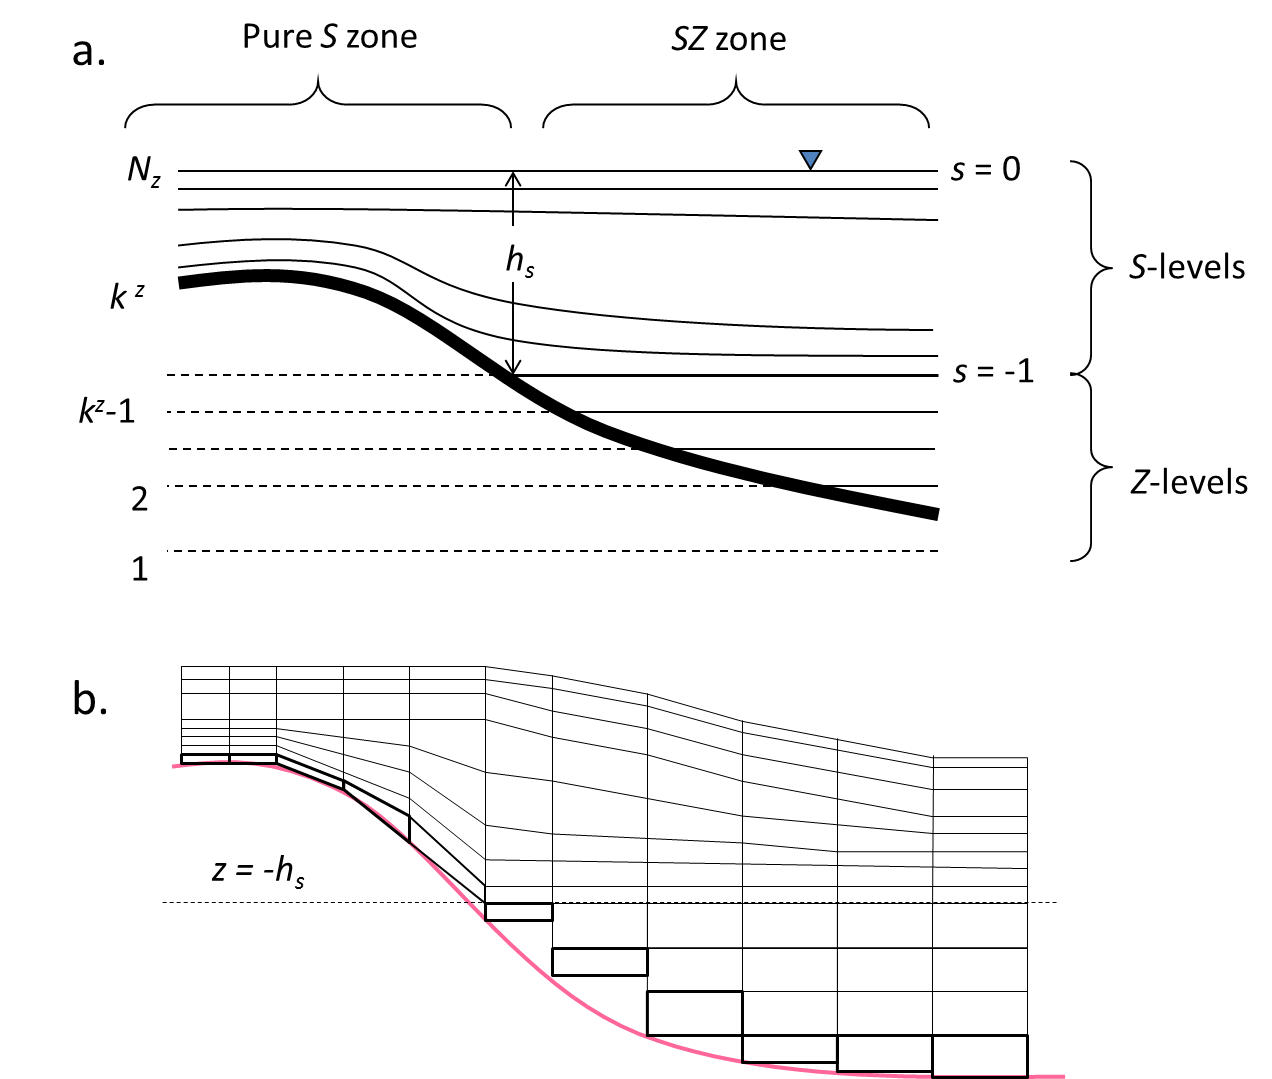
\includegraphics[scale=0.5]{image/vgrid}
	\caption{a. The hybrid coordinate system used in SELFE. S-coordinates are used above the threshold depth $h_s$,
	         while z (stairstepping) coordinates are used below. b. Vertical transect of an SZ mesh.}
	\label{fig:vgrid}
\end{figure}

Generating a good unstructured grid for SELFE requires some guidelines, and we'll elaborate on this in Section (\ref{sec-delta-mesh}). 

\subsection{Vertical mesh}
SELFE has a flexible meshing system in the vertical direction, allowing a hybrid
of Z layers below and S coordinates above as shown in Figure \ref{fig:vgrid}. 
The Z mesh has levels that are horizontal and is fixed 
at prescribed elevations, except for the partial level at the bed. This leads to 
a stairstep representation of the boundary as shown. The S coordinates \citep{Song94} are 
terrain following, with a constant number of levels between the bed (or uppermost z layer) and the free surface. 
The S grid parametrization allows the user to concentrate greater or less
density in the lower or upper boundary layers.  \gls{cmop} did extensive side-by-side 
testing of SELFE and ELCIRC, a Z-based model, and the terrain following mesh is one of the factors cited in the improved performance of SELFE.

As we shall describe in Section \ref{sec-delta-mesh}, we felt the Bay-Delta is generally shallow 
enough to avoid the $Z$ layers entirely.
The original purpose of the SZ hybrid was to avoid some of the pitfalls associated with topography conforming
meshes particularly on steep bathymetry in deep water, particularly so-called {\em hydrostatic inconsistency} and
the associated issues of inaccuracy in pressure calculations \citep{Shchepetkin05,Haney91}. Subsequent work on several basins, including the Columbia River, indicate that except in particularly steep, deep applications the pressure errors are secondary compared to the benefits of a terrain conforming mesh.

Although we are confident the pure-S approach is the best option available to us between S, Z and SZ,
we have also begun testing a vanishing quasi-sigma vertical coordinate system similar to that described by
\cite{Dukhovskoy09} in which layers disappear gradually in shallower water. Our implementation includes an
enhancement to avoid the stairstepping noted by  \cite{Dukhovskoy09}. This gridding system preserves the advantages
of bathymetry conforming coordinates while reducing pressure errors,
preserving stratification and eliminating some practical issues associated with 
over-resolution in shallow water. Such overcrowding of layers in shallow water almost always
occurs upstream if the deeper waters in the Bay are properly resolved).

Regardless of what vertical mesh option is chosen when running SELFE, the primary purpose of the mesh is to define the 
locations of the prisms in vertical space, which in the case of S coordinates changes over time with the evolution of
the water surface. This calculation is made once per time step; once that transformation is complete, the 
solver is based almost entirely on z coordinates.

\begin{figure}
	\centering
		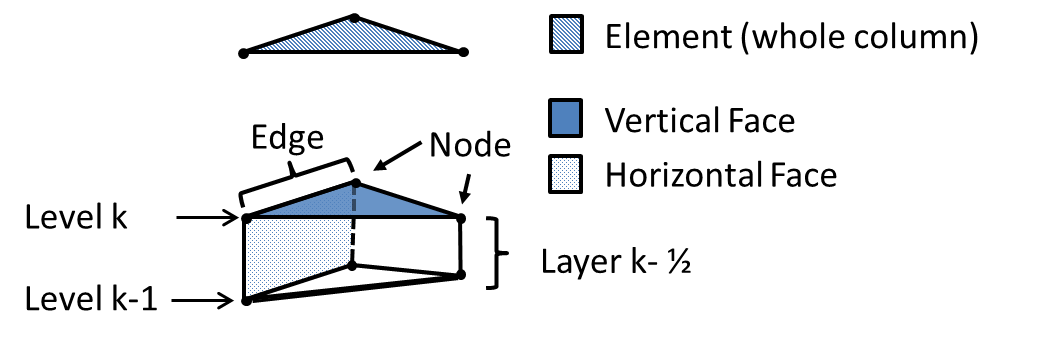
\includegraphics[scale=1.0]{image/prism}
	\caption{Nomenclature associated with a prism. Note that the term {\em element} is used for 
	the 2D horizontal component, and also for integrated quantities involving the entire water column. 
	.}
	\label{fig:prism}
\end{figure}


\subsection{Variables and mesh centerings}
Fig \ref{fig:prism} illustrates the nomenclature associated with the staggering scheme and variable locations used in SELFE. 
The surface elevation is defined at nodes, horizontal velocity at side (edges of an element) centers and whole levels (tops of prisms), tracers at prism centers (under upwind
or TVD transport schemes), and the vertical velocity at element centroids and whole levels. The staggering of variable enhances numerical stability \citep{Danilov13}. One difference to note between SELFE and other semi-implicit models
such as UnTRIM and SUNTANS is that SELFE calculates both components of velocity $(u,v)$ rather than a single
component normal to the edge. This is not relevant when calculating fluxes, but it avoids certain difficulties associated
with the Coriolis term. 

\section{Simulation steps and options}
\subsection{Outline of solution}
Details of the solution steps for the hydrostatic algorithm are given in the SELFE paper \citep{Zhang08}. 
Our goal here is only to sketch the algorithm, focusing attention on components that represent important
solver options. 

The time advance from step $n$ to step $n+1$ includes the following steps:

\begin{description}
\item[Momentum advection] The advection of momentum is handled using the \gls{elm} method. In an ELM, changes in advection are evaluated along flow paths, which means that characteristic paths have to be {\em backtracked}. 
\item[Evaluation of explicit terms] The momentum equation includes some terms that are implicit (the value
over the time step is estimated by a combination of the value at the old time $n$ and the new time $(n+1)$.
An example is friction.
Other terms, notably horizontal viscosity and Coriolis, are 
evaluated explicitly using only the value at time $n$. This 
step calculates the old time component of the implicit terms and
\item[Depth averaged mass and momentum] The depth-integrated mass and momentum equations are combined into
a single (2D) integral form and solved using the Finite Element Method. This step produces the new water surface
height $\eta^{(n+1)}$. 
\item[Horizontal velocity] is calculated algebraic from the momentum equation and new water surface algebraically
\item[Vertical closure] Vertical velocities are inferred from the horizontal ones and mass conservation.
\item[Transport] Salt and temperature are advanced using the velocity field just calculated. These will be used
in the hydrodynamics for density evaluation in the next time step
\item[Turbulence] closure is updated for use in the next time step (on a lagged basis)
\end{description}



\subsection{ELM options}
In SELFE, the momentum advection is {\em always} treated with ELM. The transport equation can be solved using ELM as well, although this is rarely done due to mass conservation issues associated with ELM. 

The ELM option treats the advection in an Eulerian-Lagrangian sense. For example, the total derivative of the velocity is approximated as:
\beq
  \frac{D u}{D t} \approx \frac{u^{n+1}-u^*}{\D t}
\eeq
where $u^n$ is the velocity at the new time step and $u^*$ is calculated 
by following a fictitious flow particle, starting at a pre-given point $\bs{x}$, backward in time and space 
(Figure \ref{fig:backtrack})
\begin{figure}
	\centering
		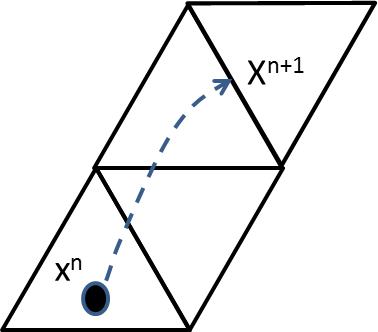
\includegraphics[scale=1.0]{image/backtrack}
	\caption{Backtracking of a fictitious particle is performed from the ending location at an edge center 
	(arrow) to the source (dot).}
	\label{fig:backtrack}
\end{figure}

The particle trajectory is determined by the characteristic equation, which moves the ficticious particle at the
the local (interpolated) velocity from the last time step.
\beq
  \frac{D \bs{x}}{D t}=\bs{u} \label{char}
\eeq

Variants of the method depend on how velocities are interpolated for purposes of backtracking and how 
quantities are interpolated at the foot of the characteristic path. 
 
In SELFE, the integration of (\ref{char}) is done using either a simpler backward Euler 
or 2nd-order Runge-Kutta scheme. To more closely follow the characteristic line, 
the integration time step is sub-divided into smaller steps.  After the foot of the characteristic line is found from (\ref{char}), $u^*$ is then interpolated using a scheme that is independent of 
the one used for backtracking. The order of interpolation function
used will determine if the ELM is diffusion (lower-order) or dispersion (higher-order) dominates the
error in the computation. In this project, the choice between lower-order interpolant was treated
as a calibration option. 


\subsection{Barotropic vs Baroclinic}
It is common, when speaking of the shallow water equations, to decompose the motion into
the barotropic and baroclinic modes. The barotropic mode is the most fundamental motion, 
and is associated with pressure gradients due to  variations in water surface height.
The baroclinic modes are induced by more complex vertical density structure
caused by salt (and temperature) differences.

In SELFE, the baroclinic and barotropic modes are toggled with a single parameter. They differ in that in Baroclinic mode, the contribution of temperature- and salinity-induced density differences is included in the momentum equations. In contrast, in Barotropic mode salt and temperature are (at most) considered passive tracers.
The turbulence closure is still calculated in 3D, but the suppression of turbulence due to stratification is not included.

One common usage pattern with SELFE is to use a sequence of barotropic-baroclinic model runs. The barotropic simulation is used in a preliminary simulation in order to calculate 3D boundary conditions (particulary the velocity) for the subsequent baroclinic analysis. Typically this is done with transport off or even, maximizing speed for the barotropic step and deliberately choosing diffusive model parameter combinations.

We believe the 3D mode can be used profitably for modeling the Delta alone with a boundary at Martinez,
particularly for studies that do not otherwise involve salt transport. The upstream part of the Delta is not stratified enough for baroclinicity to play an important role, and the cost savings of dropping salinity transport
is significant.

\subsection{Transport options}
There are three transport options available in SELFE:
\begin{enumerate}
\item \gls{elm}
\item First order upwind finite volume scheme
\item Higher accuracy \gls{tvd} finite volume scheme based on the scheme of \citet{Casulli05}
\end{enumerate}

We have already remarked that only the finite volume options are normally used. The first order and higher order TVD scheme can be hybridized on one mesh based on region or a depth-based switching criterion, and indeed the stringent \gls{cfl} time step restrictions of the TVD scheme more or less require this in shallow water. For this project, we used depth of 6m as the depth criterion and only used the TVD scheme below the confluence region.

\section{Wetting and drying}
 SELFE does not allow partial wetting and drying, and so the wetting and drying rule 
is based on full elements or edges. An element is wet if all
its 3 nodes are wet (based on the total depths there and a threshold minimum 
depth specified); otherwise it's dry. Based on this
information, a node is considered wet if and only if at least one of its surrounding
 elements is wet. Similarly, a side is 'wet'  if and only if at least 
one of its adjacent elements is wet. 

\subsection{Options}
There are two options for calculating wetting and drying at a new time step. The first consists of a simple sweep among all
nodes/sides/elements as described above. The second option is iterative starting from the shoreline position at the previous step.
The rule is applied at all shoreline nodes and adjacent elements and sides and the iteration is used to advance the shoreline from
one step to the next. At the end of iteration, a constant extrapolation scheme is used to 'project' the surface to the next
neighboring dry element. This option is designed for grids with adequate resolution so the inundation process can be tracked
accurately. For other grids, the first option should be used (as in the case of the current project).
\subsection{Implications for gridding}
\label{subsec-wet-dry-grid}
Because SELFE does not allow partial wetting and drying, the user must be careful not to grid the channel bottom too high such that
the entire channel is blocked from flow. In practice, it's best to at least use 2 nodes that are always wet in a channel, and use
extra nodes on either side to capture the wetting and drying process. However, if the other nodes are gridded too high, the side
elements may not be ever activated.

%add
\section{Hydraulic structures}
\label{sec-structures}
The term {\em hydraulic structures} refers to control structures such as tidally-operated gates, 
barriers, weirs and culverts as well as to coupled boundary conditions 
representing direct transfers of water from an outflow to an inflow boundary due to mechanisms like low head pumps. 
There are numerous gates and control structures in the San Francisco Bay-Delta. Here we describe the way structures are modeled and the formulas used to calculate flow through them. 

Hydraulic structures are represented in SCHISM as paired boundary condition (Figure \ref{fig:structmesh}). Flow is calculated based on head differences at two {\em reference nodes}, one on the nominal upstream and downstream sides of the structure (but not necessarily adjoining the structure). Once the flow is calculated, it is disaggregated as a homogenous flux boundary condition over the breadth of the structure. The boundaries are enforced using a relaxation formulation, which provides some natural ramping of flow when gates that are suddenly opened or closed. Transport is coupled between the side that is an outflow and the side that is an inflow.

\begin{figure}
	\centering
		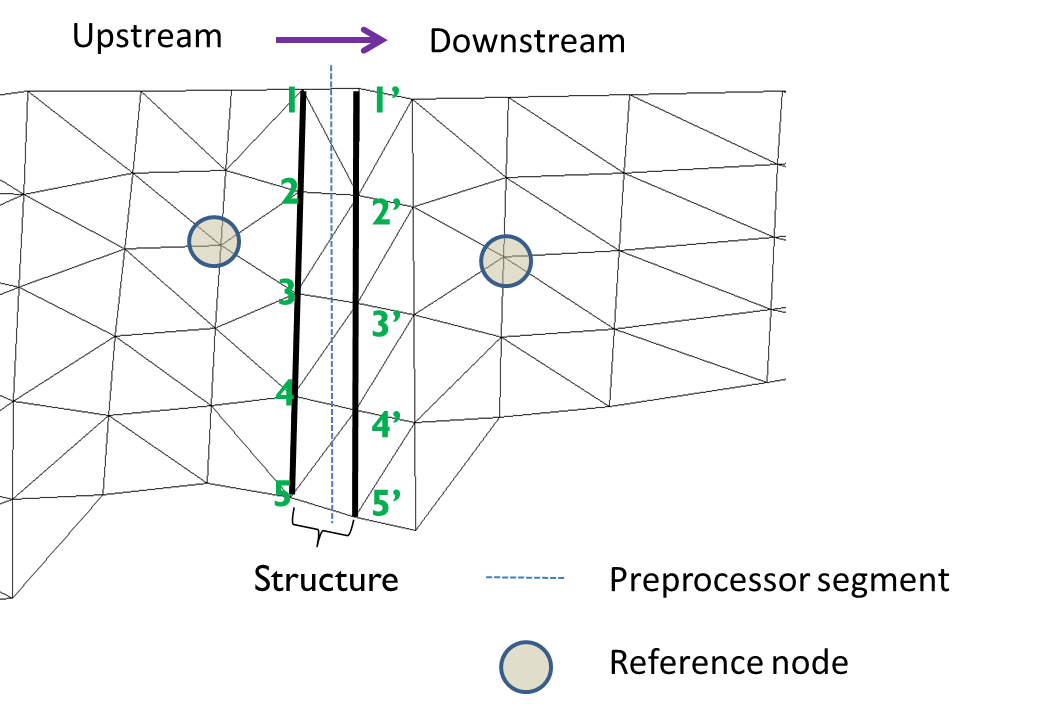
\includegraphics[scale=1]{image/struct}
	\caption{Hydraulic structure definition imposed on horizontal grid.}
	\label{fig:structmesh}
\end{figure}

A number of pre-defined flow structures are already in place covering all the cases we encountered in the Bay-Delta; with a little programming the system can easily be expanded to accommodate new structures.  
The structures we have already implemented are listed below. All of the structures admit control of key (indicated) parameters using time series. 

Structures can also be removed in SCHISM by adding 
an appropriate entry in a time series. When a structure is removed, the region between the paired boundaries reverts to the ordinary equations of motion -- ie, it is if the structure did not exist.

\subsection{Flow transfers}
\label{sec-transfer}
A flow transfer is a simple coupled boundary condition wherein a fixed flow $Q_s$ is stipulated. This flow
is imposed as an outflow boundary on one the paired boundaries and and inflow on the other. Constituent mass 
is conserved.

\begin{figure}
	\centering
		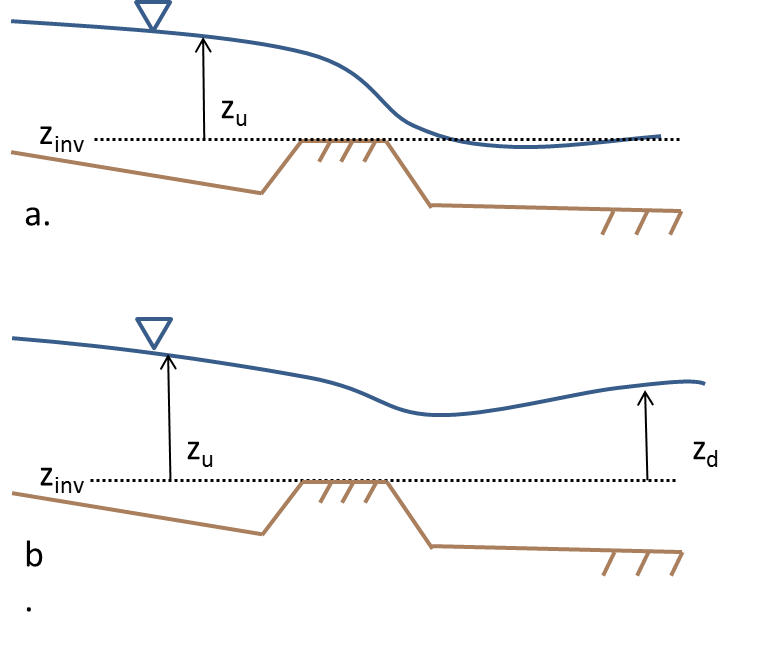
\includegraphics[scale=1]{image/weir}
	\caption{Free flowing (a) and submerged (b) weir flow cases.}
	\label{fig:weir}
\end{figure}

\subsection{Weirs}
A weir may be dry, submerged or free flowing (see Figure \ref{fig:weir}) depending on the position of the upstream
and downstream water surfaces $z_{u}$, $z_{d}$ compared to the weir invert elevation $z_{inv}$. Note that in the formulas
below, 

For the free flowing case:
$$
Q_s^f=\sgn{(z_{u} - z_{d})} C_{op} C_{f} A \sqrt{2g H}
$$
where 
\begin{align*}
&Q_s^f  &\text{free flow flow through structure (cms)} &\\
&\sgn        &\text{sign function (to induce up/downstream directionality)}  &\\
&z_u         &\text{upstream reference elevation  (m)}  &\\
&z_d         &\text{downstream reference elevation (m)}  &\\
&z_{inv}     &\text{invert elevation of the weir (m)}  &\\
&H = \max(z_u,z_d) - z_{inv}  &\text{is the energy head above the weir} &\\
&A                            &\text{area of flow (m\textsuperscript{2}) }&\\
&C_op               &\text{(directionally varying) operating coefficient (unitless)} &\\
&C_f                &\text{flow/gate coefficient (unitless)}  &\\
&g                  & \text{gravity (m/s\textsuperscript{2})} & \\
\end{align*}
For commentary on coefficients, see \cite{Rantz82}. Note that in the formulation above, the $\sqrt{2g}$
term has been kept separate and the area calculation uses water surface height. 
Furthermore, note that $z_u$ and $z_d$ are pre-assigned upstream and downstream orientations,
whereas $H$ is the energy head in the direction that is upstream of the weir in terms of actual flow.

The submerged case is derived from the free flowing case using the correction given by \citet{Villemonte47}:
\begin{align*}
Q_s^s = Q_s^f(1 - S^{1.5})^{0.385} \\
S = \frac{\min(z_u,z_d) - z_{inv}}{\max(z_u,z_d) - z_{inv}}
\end{align*}
in terms of the {\em submergence ratio} $S$.

If both sides are dry, of course $Q_s=0$ for the structure. Note that this refers to being dry with respect to the invert elevation.
The nodes may not go dry in the ordinary sense with respect to the bed -- this is the same restriction as at other SCHISM boundaries. 

\subsection{Radial gates} 
\label{sec:radial}
A radial gate is parametrized as shown in Figure \ref{fig:radial}, although at the moment we have ignored the kinetic 
energy component of upstream head (so that $H_1 = y_1$). For the case where the radial gate is completely out
of the water or the tailwater elevation is not sufficiently high to affect the upstream (submergence ratio described in the previous
section is less than $S_p=0.66$),
the gate reverts to a modified weir equation described momentarily. For the case where the radial gate is completely submerged 
(submergence ratio greater than $S_f=0.80$),
the gate is treated as an orifice as given in Section \ref{sec-orifice}.

            %diff = max_elev - min_elev
            %coef_matching_factor = sqrt(1.d0/(1.d0-PART_SUBMERGE))
            %flow = signed_coef*area*sqrt2g*sqrt(diff)
            %! now weigh the two so that the flow makes a linear transition
            %subfrac = (submerge_ratio-PART_SUBMERGE)/(FULL_SUBMERGE - PART_SUBMERGE)
            %flow = ((1.d0 - subfrac)*coef_matching_factor + subfrac)*flow
For free flow:
$$
Q_s^f = \sgn{(z_{u} - z_{d})} C_{op} C_{f} A \sqrt{2g H}
$$
and for partially submerged flow ($S_p < S \le S_f$):
$$
Q_s^p = \sgn{(z_{u} - z_{d})} C_{op} C_{f} A \sqrt{2g \left|\D z\right|}[(1-\hat{S})m+\hat{S}]
$$
where
\begin{align*}
&\hat{S}=\frac{S-S_p}{S_f-S_p} & \text{is the submergence fraction} \\
&m = \sqrt{\frac{1}{1-S_p}} & \text{is a coefficient matching factor to create a smooth transition}. \\
\end{align*}

For fully submerged flow $S>S_f$, the orifice equation is used. This is equivalent to the submerged equation with
$\hat{S}=1$.


\begin{figure}
	\centering
		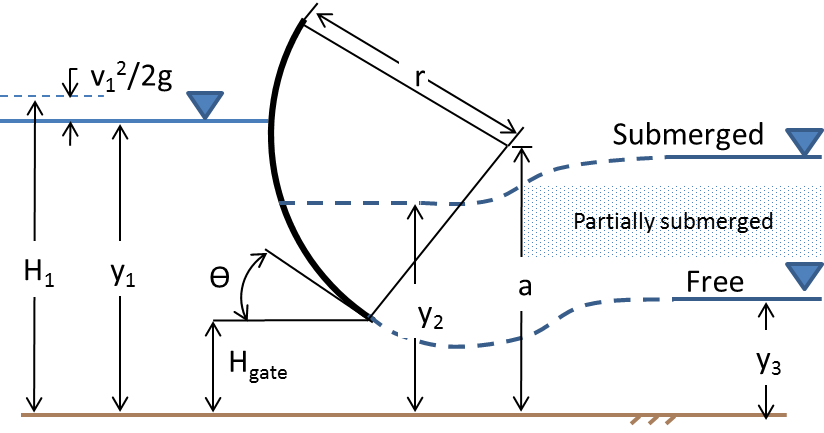
\includegraphics[scale=1]{image/radial_gate}
	\caption{Radial gate.}
	\label{fig:radial}
\end{figure}

\subsection{Radial gates with linear coefficient} 
This is an alternative radial gate formula modified from a suggestion by Tony Wahl of the USBR (personal communication) 
that was incorporated because it matches Clifton Court well. 
The rating formula is a little simpler, but the flow coefficient is a linear function of gate height:

$$
Q_s = \sgn{(z_{u} - z_{d})} C_{op} C_{f} A \sqrt{2g \left|\D z\right|}
$$
where
$$C_f = d + sR$$
is the gate coefficient linearly dependent on the ratio of gate opening to upstream head:
$$R = \min(\frac{H_{gate}}{H_1},1.0)$$
with constant and linear parameters $d$ and $s$ respectively.
Some special cases surround the term $A$, given that the top of the radial gate
may be dry or submerged.

\subsection{Orifice}
\label{sec-orifice}
The orifice option is used to model a sluice gate or flashboard or other devices that  
presents a (rectangular) apertures to flow. Flow in this case is given by:

$$
Q_{s} = \sgn{(z_{u} - z_{d})} C_{op} C_{f} A \sqrt{2g \left|\D z \right|}
$$

Some special cases surround the term $A$, given that the orifice may be dry, partially submerged or completely
submerged. Typically, the orifice equation is most useful when flow is fully submerged.

\subsection{Culverts}
A culvert is currently modeled as a circular orifice. In other words, it is the same as the orifice case
but with a different formula for $A$. This treatment neglects some of the nuances of head and tailwater control 
as described by \cite{Bodhaine68}



\section{Mass sources and sinks}
\label{sec-source}
Assuming that the extra momentum from the sources and sinks is negligible, 
we accommodate sources through the by adding them to the continuity equation (\ref{cont1}):
\beq
  \eta_t+\nabla \cdot \int_{-h}^\eta \bs{u}  = \sum_m s_m(t)\hat{S}(\bs{x}-\bs{x}_m) \label{cont2}
\eeq
where $s_m$ is the discharge, and $\hat{S}$ is a Dirac delta function defined at a series of points $\bs{x}_m$ (in the model we
assume these are located at element centroids). Note that the transport equation (\ref{tr1}) already accounts for the sources and sinks in the term $\hat{Q}$.


\section{Model-specific sources of error/uncertainty}
  \subsection{Mass conservation}
    SELFE does not explicitly enforce volume conservation (through the continuity equation), 
		due to the Galerkin \gls{fem} used in the solver. Mass
conservation for tracers is however enforced with the upwind/TVD schemes, as a consistent treatment is used for the 3D continuity
equation (\ref{3Dcon}) and the transport fluxes.
	\subsection{Vertical closure for flow over topography}
    This error is related to the volume conservation error shown above. The horizontal divergence drives the vertical velocity, which is calculated starting from the bottom b.c. and progressing upward. The mismatch between the calculated vertical
velocity at the surface and the b.c. there is the closure error. The error can be large when the bottom slope is large (e.g., Golden
Gate). Judicious gridding and choice of vertical grid can alleviate this error somewhat. 

   Note that even if the volume is perfectly conserved, the vertical velocity may still become too large at the surface due to other
reasons as explained in Wolfram and Fringer (2013).
	\subsection{Shallow water and friction}
    The use of a large bottom friction in shallow areas in SELFE3D can lead to parasitic oscillations due to spurious wetting and
drying. This is particularly the case when the channel is narrow and under-resolved. In this case, the 3D model tends to generate
large vertical shear as the flow is being blocked. Note that SELFE2D does not have this issue as a 2D model cannot allow vertical
shear. 
    Obviously this has implication for gridding. A simple work-around is to ramp the friction down in the shallow areas to alleviate
the shear. This approach has worked reasonably well for Bay-Delta domain. 
	\subsection{Diffusion-dispersion characteristics}
  SELFE has a myriad of schemes inside. Some schemes are more diffusive than others. An example is the interpolation schemes used in
ELM. Another example is the scheme used to convert side-based velocity from node-based velocity. This can be done using a simple
weighted averaging scheme which is more diffusive, or using the linear conforming or non-conforming shape function inside each
surrounding element before averaging. The latter is more dispersive, and requires a 5-point Shapiro filter to filter out spurious
sub-grid modes. 
